% Options for packages loaded elsewhere
\PassOptionsToPackage{unicode}{hyperref}
\PassOptionsToPackage{hyphens}{url}
%
\documentclass[
  ignorenonframetext,
]{beamer}
\usepackage{pgfpages}
\setbeamertemplate{caption}[numbered]
\setbeamertemplate{caption label separator}{: }
\setbeamercolor{caption name}{fg=normal text.fg}
\beamertemplatenavigationsymbolsempty
% Prevent slide breaks in the middle of a paragraph
\widowpenalties 1 10000
\raggedbottom
\setbeamertemplate{part page}{
  \centering
  \begin{beamercolorbox}[sep=16pt,center]{part title}
    \usebeamerfont{part title}\insertpart\par
  \end{beamercolorbox}
}
\setbeamertemplate{section page}{
  \centering
  \begin{beamercolorbox}[sep=12pt,center]{part title}
    \usebeamerfont{section title}\insertsection\par
  \end{beamercolorbox}
}
\setbeamertemplate{subsection page}{
  \centering
  \begin{beamercolorbox}[sep=8pt,center]{part title}
    \usebeamerfont{subsection title}\insertsubsection\par
  \end{beamercolorbox}
}
\AtBeginPart{
  \frame{\partpage}
}
\AtBeginSection{
  \ifbibliography
  \else
    \frame{\sectionpage}
  \fi
}
\AtBeginSubsection{
  \frame{\subsectionpage}
}

\usepackage{amsmath,amssymb}
\usepackage{iftex}
\ifPDFTeX
  \usepackage[T1]{fontenc}
  \usepackage[utf8]{inputenc}
  \usepackage{textcomp} % provide euro and other symbols
\else % if luatex or xetex
  \usepackage{unicode-math}
  \defaultfontfeatures{Scale=MatchLowercase}
  \defaultfontfeatures[\rmfamily]{Ligatures=TeX,Scale=1}
\fi
\usepackage{lmodern}
\ifPDFTeX\else  
    % xetex/luatex font selection
\fi
% Use upquote if available, for straight quotes in verbatim environments
\IfFileExists{upquote.sty}{\usepackage{upquote}}{}
\IfFileExists{microtype.sty}{% use microtype if available
  \usepackage[]{microtype}
  \UseMicrotypeSet[protrusion]{basicmath} % disable protrusion for tt fonts
}{}
\makeatletter
\@ifundefined{KOMAClassName}{% if non-KOMA class
  \IfFileExists{parskip.sty}{%
    \usepackage{parskip}
  }{% else
    \setlength{\parindent}{0pt}
    \setlength{\parskip}{6pt plus 2pt minus 1pt}}
}{% if KOMA class
  \KOMAoptions{parskip=half}}
\makeatother
\usepackage{xcolor}
\newif\ifbibliography
\setlength{\emergencystretch}{3em} % prevent overfull lines
\setcounter{secnumdepth}{-\maxdimen} % remove section numbering


\providecommand{\tightlist}{%
  \setlength{\itemsep}{0pt}\setlength{\parskip}{0pt}}\usepackage{longtable,booktabs,array}
\usepackage{calc} % for calculating minipage widths
\usepackage{caption}
% Make caption package work with longtable
\makeatletter
\def\fnum@table{\tablename~\thetable}
\makeatother
\usepackage{graphicx}
\makeatletter
\def\maxwidth{\ifdim\Gin@nat@width>\linewidth\linewidth\else\Gin@nat@width\fi}
\def\maxheight{\ifdim\Gin@nat@height>\textheight\textheight\else\Gin@nat@height\fi}
\makeatother
% Scale images if necessary, so that they will not overflow the page
% margins by default, and it is still possible to overwrite the defaults
% using explicit options in \includegraphics[width, height, ...]{}
\setkeys{Gin}{width=\maxwidth,height=\maxheight,keepaspectratio}
% Set default figure placement to htbp
\makeatletter
\def\fps@figure{htbp}
\makeatother

\makeatletter
\makeatother
\makeatletter
\makeatother
\makeatletter
\@ifpackageloaded{caption}{}{\usepackage{caption}}
\AtBeginDocument{%
\ifdefined\contentsname
  \renewcommand*\contentsname{Table of contents}
\else
  \newcommand\contentsname{Table of contents}
\fi
\ifdefined\listfigurename
  \renewcommand*\listfigurename{List of Figures}
\else
  \newcommand\listfigurename{List of Figures}
\fi
\ifdefined\listtablename
  \renewcommand*\listtablename{List of Tables}
\else
  \newcommand\listtablename{List of Tables}
\fi
\ifdefined\figurename
  \renewcommand*\figurename{Figure}
\else
  \newcommand\figurename{Figure}
\fi
\ifdefined\tablename
  \renewcommand*\tablename{Table}
\else
  \newcommand\tablename{Table}
\fi
}
\@ifpackageloaded{float}{}{\usepackage{float}}
\floatstyle{ruled}
\@ifundefined{c@chapter}{\newfloat{codelisting}{h}{lop}}{\newfloat{codelisting}{h}{lop}[chapter]}
\floatname{codelisting}{Listing}
\newcommand*\listoflistings{\listof{codelisting}{List of Listings}}
\makeatother
\makeatletter
\@ifpackageloaded{caption}{}{\usepackage{caption}}
\@ifpackageloaded{subcaption}{}{\usepackage{subcaption}}
\makeatother
\makeatletter
\@ifpackageloaded{tcolorbox}{}{\usepackage[skins,breakable]{tcolorbox}}
\makeatother
\makeatletter
\@ifundefined{shadecolor}{\definecolor{shadecolor}{rgb}{.97, .97, .97}}
\makeatother
\makeatletter
\makeatother
\makeatletter
\makeatother
\ifLuaTeX
  \usepackage{selnolig}  % disable illegal ligatures
\fi
\IfFileExists{bookmark.sty}{\usepackage{bookmark}}{\usepackage{hyperref}}
\IfFileExists{xurl.sty}{\usepackage{xurl}}{} % add URL line breaks if available
\urlstyle{same} % disable monospaced font for URLs
\hypersetup{
  pdftitle={Public Policy Analysis},
  pdfauthor={Krisna Gupta},
  hidelinks,
  pdfcreator={LaTeX via pandoc}}

\title{Public Policy Analysis}
\subtitle{A Discussion}
\author{Krisna Gupta}
\date{June 21, 2023}
\institute{Center for Indonesian Policy Studies}

\begin{document}
\frame{\titlepage}
\ifdefined\Shaded\renewenvironment{Shaded}{\begin{tcolorbox}[frame hidden, interior hidden, sharp corners, borderline west={3pt}{0pt}{shadecolor}, boxrule=0pt, breakable, enhanced]}{\end{tcolorbox}}\fi

\begin{frame}{I Made Krisna}
\protect\hypertarget{i-made-krisna}{}
\begin{columns}[T]
\begin{column}{0.4\textwidth}
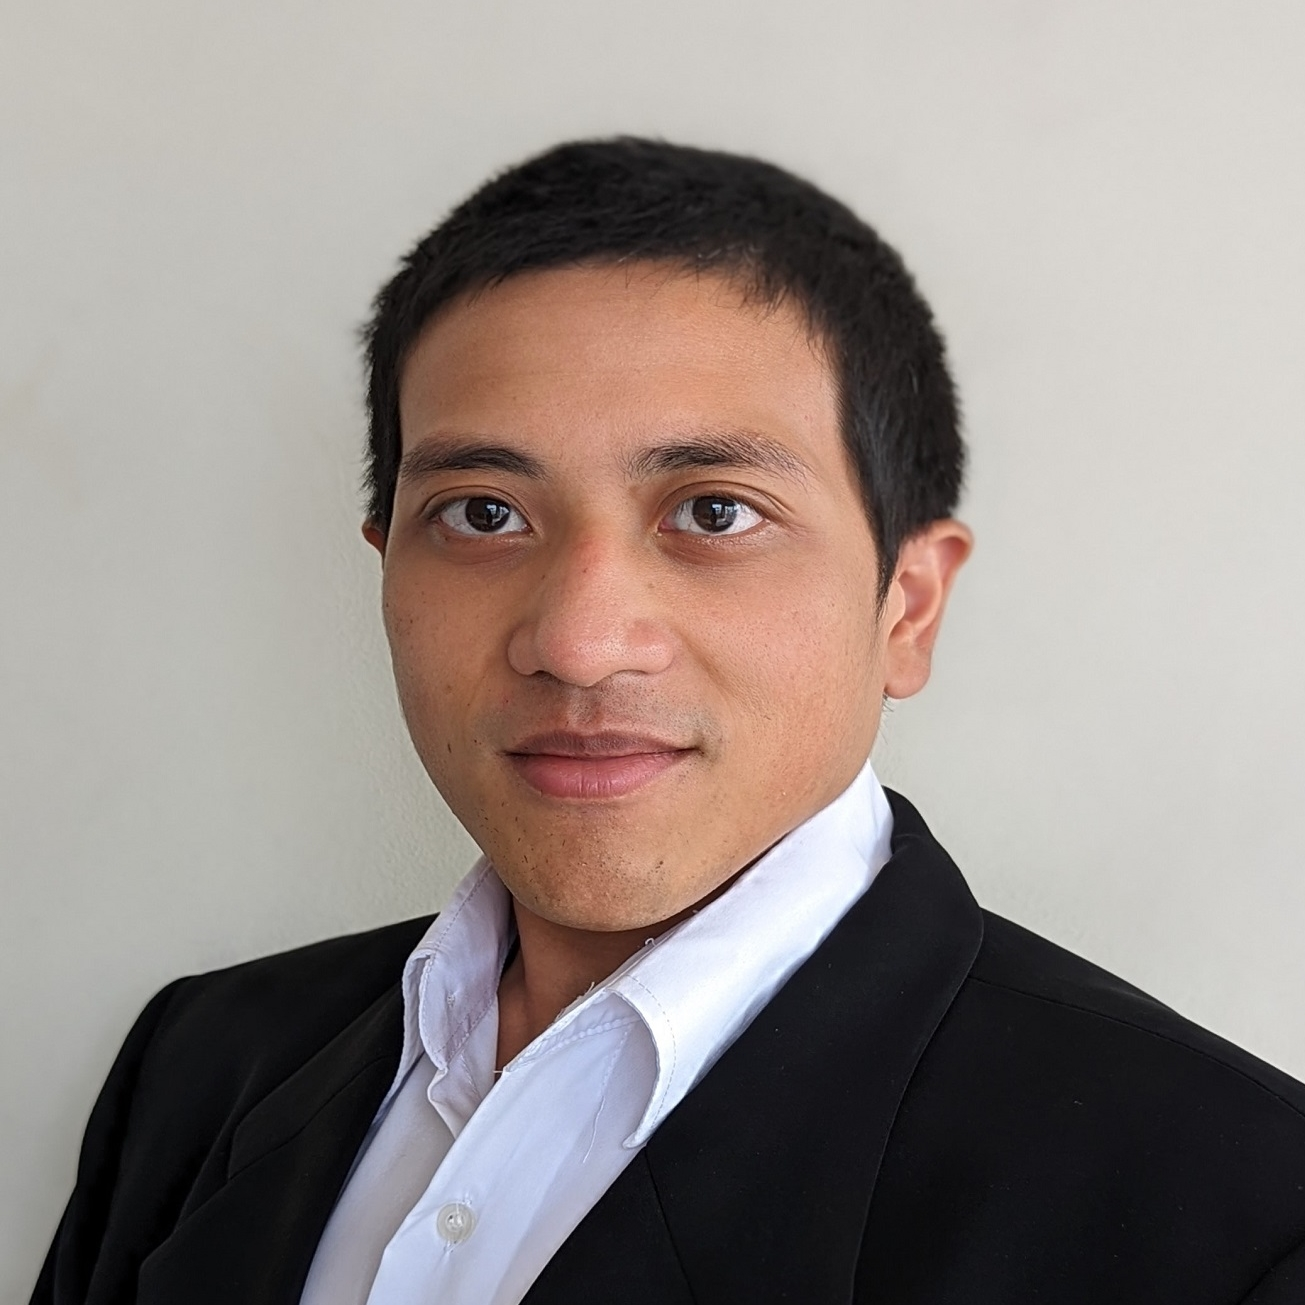
\includegraphics{cips_files/mediabag/foto_krisna.jpg}
\end{column}

\begin{column}{0.6\textwidth}
\begin{itemize}
\item
  Sering dipanggil Imed
\item
  Full-time lecturer di Politeknik APP
\item
  Part-time lecturer di Universitas Indonesia
\item
  Master degree in economics UI/VU
\item
  \href{https://crawford.anu.edu.au/people/phd/krisna-gupta}{PhD in
  economics} di Australian National University

  \begin{itemize}
  \tightlist
  \item
    \href{https://openresearch-repository.anu.edu.au/handle/1885/270149}{thesis}
    tentang industri dan perdagangan di Indonesia.
  \end{itemize}
\item
  Associate researcher di
  \href{https://www.cips-indonesia.org/about?lang=id}{Center for
  Indonesian Policy Studies}.

  \begin{itemize}
  \tightlist
  \item
    Policy paper terakhir tentang
    \href{https://www.cips-indonesia.org/publications/perdagangan-untuk-pemulihan-ekonomi\%3A-kebijakan-impor-untuk-mendukung-sektor-makanan-dan-minuman-indonesia}{GVC
    di industri makanan}
  \end{itemize}
\item
  Selengkapnya di
  \href{https://imedkrisna.github.io/}{imedkrisna.github.io}

  \begin{itemize}
  \tightlist
  \item
    blog di \href{https://www.krisna.or.id/}{krisna.or.id}
  \item
    twitter di \href{https://www.twitter.com/imedkrisna}{@imedkrisna}
  \end{itemize}
\end{itemize}
\end{column}
\end{columns}
\end{frame}

\begin{frame}{Content}
\protect\hypertarget{content}{}
\begin{itemize}
\item
  Why economics?
\item
  What to look for in writing a policy piece.
\item
  Some usual problems according to my experience.
\end{itemize}
\end{frame}

\begin{frame}{Your expectation?}
\protect\hypertarget{your-expectation}{}

\includegraphics[width=2.08333in,height=2.08333in]{qr.png}
\end{frame}

\begin{frame}{Basic assumption}
\protect\hypertarget{basic-assumption}{}
\begin{itemize}
\item
  No economics and/or mathematics background.
\item
  Some experience in CIPS' work.
\item
  chance is, I can learn from you. So don't be shy.
\end{itemize}
\end{frame}

\begin{frame}{Why Economics}
\protect\hypertarget{why-economics}{}
\begin{itemize}
\item
  Economics is NOT about (just) money!
\item
  Economics is a study of optimization: how to get the best under
  constraints.

  \begin{itemize}
  \item
    The same with engineers!
  \item
    We use very similar tools!
  \end{itemize}
\item
  Increasingly, economics also do empirics!
\end{itemize}
\end{frame}

\begin{frame}{Theory vs Empirics}
\protect\hypertarget{theory-vs-empirics}{}
\begin{itemize}
\item
  Theory: If X leads to Y while Z does not lead to Y, then lets do X.
\item
  Does X really lead to Y while Z does not?
\item
  The first is the optimization part, the second is the empirical part.
\item
  But stil, relationship between Xs \& Ys is what interests all
  economists.
\end{itemize}
\end{frame}

\begin{frame}{Some questions}
\protect\hypertarget{some-questions}{}
\begin{itemize}
\item
  How to best tackle climate change?
\item
  Is minimum wage good?
\item
  Should we ban trade to industrialize?
\item
  How to best feed our people?
\item
  Should we invest in school or road?
\end{itemize}
\end{frame}

\begin{frame}{About economics}
\protect\hypertarget{about-economics}{}
\begin{itemize}
\item
  Some of my blogpost to get a glympse of what economists do:

  \begin{itemize}
  \item
    \href{https://www.krisna.or.id/post/surga/}{Consumption-saving
    decision}
  \item
    \href{https://www.krisna.or.id/post/jorr/}{how to set the price on
    toll road}
  \item
    \href{https://www.krisna.or.id/post/hitektrade/}{FDI, trade and
    industry policy}
  \end{itemize}
\item
  Naturally, economists often specialize more on issues.

  \begin{itemize}
  \tightlist
  \item
    I'm more on trade, industry, investment. Knows next to nothing about
    education \& welfare program issues.
  \end{itemize}
\end{itemize}
\end{frame}

\begin{frame}{Why people make choices}
\protect\hypertarget{why-people-make-choices}{}
\begin{itemize}
\item
  The main reason is resources' scarcity.
\item
  resource = anything you use to get what you want.
\item
  mainstream resources are money; Given 4k trilyun APBN, what program
  should we finance?
\item
  But other resources are important too: time, people/institutions,
  inflation.
\end{itemize}
\end{frame}

\begin{frame}{Opportunity cost}
\protect\hypertarget{opportunity-cost}{}
\begin{itemize}
\item
  The true cost of something is its possible other uses. Money is the
  least of our concern.
\item
  The cost of having holiday, for example, is the money \& time you
  could otherwise use to join a short course.
\item
  The cost of doing an S1:

  \begin{itemize}
  \item
    Go straight to work, get experiences \& money
  \item
    Do other degree
  \item
    enjoy life
  \end{itemize}
\item
  I daresay opportunity cost is the core concept of economics!
\end{itemize}
\end{frame}

\begin{frame}{Thinking at the margin}
\protect\hypertarget{thinking-at-the-margin}{}
\begin{itemize}
\item
  The principle of opportunity cost leads to a marginal thinking
\item
  understand the status quo, then think if it can be (marginally)
  improved.
\item
  e.g., say you have 2 hours to spent on work or play. how to divide?

  \begin{itemize}
  \item
    depends: when's the work deadline?
  \item
    if you work for another 30 minutes, would that help with work?
  \end{itemize}
\end{itemize}
\end{frame}

\begin{frame}{Specialization \& trade}
\protect\hypertarget{specialization-trade}{}
\begin{itemize}
\item
  During your daily time, you make decisions on allocating how much time
  to study and to cook, among other things.
\item
  Since you will die if you don't eat, you can't allocate 0 hour to
  cook.
\item
  On the other hand, there are those who are very good cook and will
  cook for you for a little money.
\item
  In this case, it may be better if you spend 0 hour to cook, and order
  food from these chefs.
\item
  Trade is the reason why I can study economics: I don't have to study
  how to be a doctor. I will just go to the hospital if I need a medical
  service.
\end{itemize}
\end{frame}

\begin{frame}{SPecialization \& trade}
\protect\hypertarget{specialization-trade-1}{}
\begin{itemize}
\item
  Extending to firm level:

  \begin{itemize}
  \item
    Why build our own office suit if we can buy microsoft office?
  \item
    Why build our own server if there's AWS, Biznet, others?
  \end{itemize}
\item
  Easily extending this to country level:

  \begin{itemize}
  \tightlist
  \item
    Japan's capital \& labor are mobilized to make cars cuz they get
    less if they plant palm oil.
  \end{itemize}
\item
  Remember: export is beneficial because we can import from the revenue!
\end{itemize}
\end{frame}

\begin{frame}{Typical problem}
\protect\hypertarget{typical-problem}{}
\begin{itemize}
\item
  Most policy makers \& policy analysts are stumble in the trade
  argument because they often forgot about \textbf{resource constraints}
  and \textbf{opportunity cost}.

  \begin{itemize}
  \tightlist
  \item
    leads to a macro-policy which aims at increasing
    \textbf{everything}.
  \end{itemize}
\item
  our land, workforce, APBN, etc are limited.
\item
  Even if you have a lot of resources, for example, the extra money
  could be better spent to grow one thing.
\end{itemize}
\end{frame}

\begin{frame}{Political context}
\protect\hypertarget{political-context}{}
\begin{itemize}
\item
  There is almost no policy that's not biased: benefits some
  sub-population while hurts others.

  \begin{itemize}
  \item
    Agriculture Imports hurts farmers while helps consumers and
    industrialists.
  \item
    Scholarships benefit smart individuals \& high-skilled industries.
  \item
    All subsidies benefit targeted groups at the expense of taxpayers.
  \end{itemize}
\item
  Economists often focuses on generalization and leaning toward policies
  that improves \textbf{aggregate welfare}
\end{itemize}
\end{frame}

\begin{frame}{Equilibrium}
\protect\hypertarget{equilibrium}{}
\begin{itemize}
\item
  When there is an incentive to do something, there will be more and
  more people exploit it.
\item
  As more people do it, the incentive decreases to a point where it is
  not worth it anymore.
\item
  examples:

  \begin{itemize}
  \item
    City becomes more crowded (and costly to live in).
  \item
    Countries' economic growth reduced after they get rich.
  \end{itemize}
\item
  Movement towards equilibrium, however, varies.

  \begin{itemize}
  \tightlist
  \item
    short run vs long run,individual vs aggregate.
  \end{itemize}
\end{itemize}
\end{frame}

\begin{frame}{Conclusion}
\protect\hypertarget{conclusion}{}
\begin{itemize}
\item
  Main principles: scarcity, opportunity cost, marginal thinking, \&
  equilibrium.
\item
  Economics gets much more complicated that this.
\item
  The principle, however, remains the same (more or less)
\end{itemize}
\end{frame}

\begin{frame}{Discussion}
\protect\hypertarget{discussion}{}
Consider a country called Kuvukiland which has 2 industries: wheat and
bread, and 3 classes of people: consumers, farmers who work in the wheat
industry, and bakers who work in the bread industry. Consumers eat only
bread \& all wheat goes to bakers. Technology is simple: 1 bushel of
wheat -\textgreater{} 1 loaf of bread. Price bread = price wheat.

With no trade, farmers produce 8 ton wheat at P=7000. With trade,
Kuvukiland can import with international prices at P=6000, demand rises
to 10 ton, but at that price, farmers only produce 6 ton. 4 ton are
imported.

Discuss: is trade better? Who benefits? If there's a ballot, who will
vote for free trade?
\end{frame}

\begin{frame}{Writing a policy paper}
\protect\hypertarget{writing-a-policy-paper}{}
\begin{itemize}
\item
  This is not a writing drill. Everybody has their own style.
\item
  However, there are some things that you may want to have in your
  writing.
\item
  Don't forget to keep the principle in our previous learning in your
  mind while doing this.
\end{itemize}
\end{frame}

\begin{frame}{Public Policy Principle}
\protect\hypertarget{public-policy-principle}{}
\begin{itemize}
\item
  We often write something theoretical
  \href{https://www.cips-indonesia.org/publications/the-advent-of-a-new-trade-governance-after-the-omnibus-law\%3A-neraca-komoditas}{(like
  this for example)} but also something more empirics
  \href{https://www.cips-indonesia.org/publications/technology-and-knowledge-transfers-to-dairy-farms\%3A-private-sector-contribution-to-improve-milk-production}{(like
  this for example)}
\item
  Well, in reality, it is not so useful differentiating the two. We
  often just mix them.
\item
  However, you can see the pattern of these works are somewhat similar.
\end{itemize}
\end{frame}

\begin{frame}{What to look for?}
\protect\hypertarget{what-to-look-for}{}
When we write about policy, aim for these things:

\begin{enumerate}
\item
  Problem definition
\item
  Policy targets
\item
  Policy assessments
\item
  Assess alternative options
\end{enumerate}
\end{frame}

\begin{frame}{Problem definition}
\protect\hypertarget{problem-definition}{}
\begin{itemize}
\item
  Why the regulation is needed? The reason often boils down to the
  presence of market failure, inefficient prior regulations, or new
  targets.
\item
  Find this in a ``menimbang'' part, sometimes at ``pasal 2'', but
  sometimes in the media.
\item
  Some regulations try to tackle more than one problem, so list them
  accordingly.
\item
  Your paper may or may not contain regulation, but the problem
  definition is a must-have.
\item
  See if these problems can be translated into policy targets.
\end{itemize}
\end{frame}

\begin{frame}{Policy targets}
\protect\hypertarget{policy-targets}{}
\begin{itemize}
\item
  If you write on a particular policy, first you must tell readers what
  it is and how does it work.
\item
  You must state boldly what it tries to achieve, then you must focus
  these targets.
\item
  Identify whether you can relatively easily inspect those targets.
\item
  Identify which target the government say it has been achieved, and
  check whether it's true.
\item
  If you're not studying a particular policy, then state these targets
  in your policy recommendations.
\end{itemize}
\end{frame}

\begin{frame}{Policy target}
\protect\hypertarget{policy-target}{}
\begin{figure}

{\centering 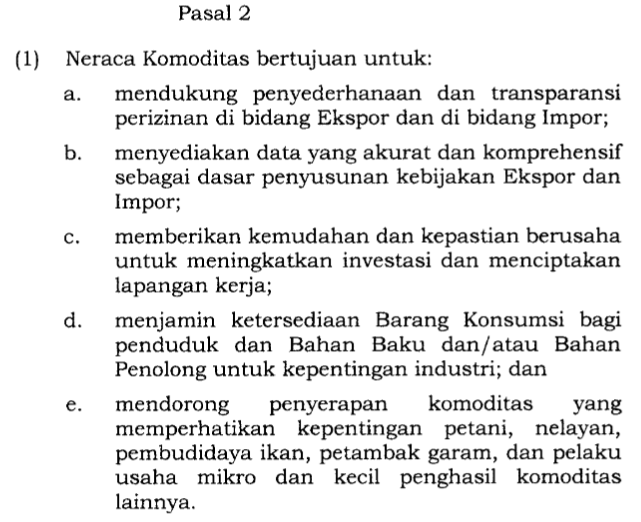
\includegraphics{goal.png}

}

\caption{contoh di Perpres 32/2022 tentang Neraca Komoditas}

\end{figure}
\end{frame}

\begin{frame}{Policy assessment}
\protect\hypertarget{policy-assessment}{}
\begin{itemize}
\item
  The assessment part usually straightforward. See if you can argue or
  find data on it.

  \begin{itemize}
  \item
    make sure you understand the mechanism from the policy to the
    result.
  \item
    e.g.~how CPO exports (the policy) leads to lower domestic prices?
  \end{itemize}
\item
  If you know the mechanism, it is easier to find the gap:

  \begin{itemize}
  \tightlist
  \item
    CPO exports failed amid wrong assumption:
    \(P\downarrow \Rightarrow Q\downarrow\)
  \end{itemize}
\item
  Assess qualitatively if finding hard data is not easy.
\item
  as long as you focus on the policy \(\rightarrow\) target mechanism,
  should be fine.
\end{itemize}
\end{frame}

\begin{frame}{Check/offer alternatives}
\protect\hypertarget{checkoffer-alternatives}{}
\begin{itemize}
\item
  Try to hypothesize policy alternatives, and see if it would have
  worked better!

  \begin{itemize}
  \item
    Always remember the context around the policy!
  \item
    No policy IS a policy!
  \end{itemize}
\item
  You can try to look for papers or studies on similar policy under
  different context (usually policies in different countries).
\item
  Approach with Cost-Benefit!

  \begin{itemize}
  \item
    Think of cost as not just money.opportunity cost guys!
  \item
    Benefit also lies beyond money.
  \end{itemize}
\end{itemize}
\end{frame}

\begin{frame}{Usual problems}
\protect\hypertarget{usual-problems}{}
\begin{itemize}
\item
  Target is often not realistic / too broad. (e.g., Free Trade Agreement
  -\textgreater{} higher exports)
\item
  Correlation is not the same as causation:

  \begin{itemize}
  \item
    reverse causality (X causes Y or Y causes X).
  \item
    spurious correlation (X \& Y moves together \(\neq\) one cause
    another).
  \item
    no counterfactual (Try to theorize the counterfactual or better yet
    use causal inference techniques)
  \end{itemize}
\end{itemize}
\end{frame}

\begin{frame}{Usual problems}
\protect\hypertarget{usual-problems-1}{}
\begin{itemize}
\item
  You must also think in a power balance / political context (vested
  interests):

  \begin{itemize}
  \item
    Which class / part of populations gets the benefit? Which one bear
    the cost?
  \item
    Who would help your advocation, who will block it?
  \item
    Almost all policy is about ``keberpihakan''
  \end{itemize}
\item
  ``Government'' is a really broad term. In truth, they're vastly
  different between \& within Ministries/Agencies: interests, KPI,
  qualities, party, etc.

  \begin{itemize}
  \tightlist
  \item
    their cooperation can't be taken for granted.
  \end{itemize}
\end{itemize}
\end{frame}

\begin{frame}{Usual problems}
\protect\hypertarget{usual-problems-2}{}
\begin{itemize}
\item
  The consequence of a target is often unclear for policy makers.

  \begin{itemize}
  \tightlist
  \item
    Blocking milk imports -\textgreater{} dwarves manufacturing growth
    (well this is partly vested interests)
  \end{itemize}
\item
  The consequence of a target may be worth it

  \begin{itemize}
  \item
    Maybe its okay to be poor as long as we can call ourselves
    agriculture nation?
  \item
    A grand mosque maybe more important than good schools?
  \end{itemize}
\item
  We assess, but it's political decision in the end.
\end{itemize}
\end{frame}

\begin{frame}{Usual problems}
\protect\hypertarget{usual-problems-3}{}
\begin{itemize}
\item
  Context matter heavily, especially institutional capacity.

  \begin{itemize}
  \item
    In developed countries, subsidies work well because almost everyone
    has bank accounts.
  \item
    Finance is less of a problem in developed countries.
  \item
    Corruption. I don't have to say more.
  \item
    Governments often didn't know what's a reform mean.
  \end{itemize}
\item
  We often needs to be creative because we face different constraints
  compared to other countries.
\end{itemize}
\end{frame}

\begin{frame}{Bottom line}
\protect\hypertarget{bottom-line}{}
\begin{itemize}
\item
  Look for the actual problems \& the policy targets
\item
  Assess for alternatives \& look for typical cause of why a policy
  fails (or potentially fails)
\item
  Use hard data if you can, assess qualitatively if you can't.
\item
  Remember to understand the political context behind every policy.
\end{itemize}
\end{frame}

\begin{frame}{Exercise}
\protect\hypertarget{exercise}{}
\begin{itemize}
\tightlist
\item
  Can you identify those points in the policy analysis must-haves? Use
  whatever policy paper/brief you're familiar with or use
  \href{https://c95e5d29-0df6-4d6f-8801-1d6926c32107.usrfiles.com/ugd/c95e5d_7735b11428c94102a3ff186b55058b2a.pdf}{this
  piece}
\end{itemize}
\end{frame}

\begin{frame}{Last slide}
\protect\hypertarget{last-slide}{}
\begin{itemize}
\item
  Thanks for your participations!
\item
  If you're interested learning more on basic economics, check out my
  course for Universitas Petra's undergrad program
  \href{https://www.krisna.or.id/courses/econ101/}{here}
\item
  My policy part is taken mostly from World Bank's RIA analysis which
  can be
  \href{https://www.google.com/url?sa=t\&rct=j\&q=\&esrc=s\&source=web\&cd=\&ved=2ahUKEwid5qjEvs7_AhUTXGwGHW2cAuwQFnoECA0QAQ\&url=https\%3A\%2F\%2Fdocuments1.worldbank.org\%2Fcurated\%2Fen\%2F905611520284525814\%2FGlobal-Indicators-of-Regulatory-Governance-Worldwide-Practices-of-Regulatory-Impact-Assessments.pdf\&usg=AOvVaw1iey7-rf-LV1TDlVYpYWe7\&opi=89978449}{downloaded
  here}
\end{itemize}
\end{frame}



\end{document}
